\documentclass{beamer}

% \usepackage{beamerthemesplit} // Activate for custom appearance

\title{Introduction to Bayesian Inference}
\author{Frank Wood}
\date{\today}

\newcommand{\comment}[1]{}
\newcommand{\ponedec}{\mathcal{P}^\downarrow_1}
\newcommand{\pone}{\mathcal{P}_1}
\newcommand{\rank}[1]{\mathrm{RANK}\left[#1\right]}
\newcommand{\E}[1]{\mathrm{E}\left[#1\right]}
\newcommand{\py}{\mathcal{PY}}
\newcommand{\iid}{iid.}
\newcommand{\drawiid}{\stackrel{\text{iid}}{\sim}}
\newcommand{\vect}[1]{\mathbf{#1}}
\newcommand{\indicator}[1]{\text{I}\left[ #1 \right]}
\newcommand{\pdcoag}{PD(d_1,0)-\text{COAG}}
\newcommand{\todo}{\textbf{*TODO*}}
\newcommand{\igram}{\text{$\infty$-gram}}
\newcommand{\Prob}{\text{P}}

\def\mm{sequence memoizer }
\def\MM{SM }

\def\pibf{{\boldsymbol{\pi}}}
\def\kapbf{\boldsymbol{\kappa}}
\def\taubf{\boldsymbol{\tau}}
\def\thebf{\boldsymbol{\theta}}
\def\rhobf{\boldsymbol{\rho}}
\def\phibf{\boldsymbol{\phi}}
\def\pbf{\mathbf{p}}
\def\qbf{\mathbf{q}}
\def\sbf{\mathbf{s}}
\def\tbf{\mathbf{t}}
\def\ybf{\mathbf{y}}
\def\wbf{\mathbf{w}}
\def\xbf{\mathbf{x}}
\def\rbf{\mathbf{r}}
\def\tbf{\mathbf{t}}
\def\kbf{\mathbf{k}}
\def\Xbf{\mathbf{X}}
\def\0bf{\mathbf{0}}
\def\Ibf{\mathbf{I}}
\def\phibf{\mathbf{\phi}}
\def\Phibf{\mathbf{\Phi}}
\def\disteq{{\stackrel{D}{=}}}
\def\EE{{\mathbb{E}}}

\def\phiv{\varphi}
\def\phivbf{\boldsymbol{\varphi}}

\def\Ocal{\mathcal{O}}

\DeclareMathOperator*{\Bet}{Beta}
\DeclareMathOperator{\coag}{COAG}
\DeclareMathOperator{\frag}{FRAG}
\DeclareMathOperator*{\rnk}{RANK}
\DeclareMathOperator*{\gem}{GEM}
\DeclareMathOperator*{\pd}{PD}
\DeclareMathOperator*{\gd}{GDir}
\DeclareMathOperator*{\Dir}{Dir}


\begin{document}

\frame{\titlepage}

\section[Outline]{}
\frame{\tableofcontents}

\section{Introduction}
\subsection{Overview of Topics}

\section{Bayesian Analysis}
\subsection{Single Parameter Model}
\frame[t] {% slide 1
 \frametitle{Bayesian Analysis Recipe}

Bayesian data analysis can be described as a three step process
\begin{enumerate}
\item Set up a full (generative) probability model
\item Condition on the observed data to produce a posterior distribution, the conditional distribution of the unobserved quantities of interest (parameters or functions of the parameters, etc.)
\item Evaluate the goodness of the model
\end{enumerate}
}

\frame[t] {% slide 2
 \frametitle{Philosophy}

Gelman, ``Bayesian Data Analysis''
\begin{quotation}\small
A primary motivation for believing Bayesian thinking important is that it facilitates a common-sense interpretation of statistical conclusions.  For instance, a Bayesian (probability) interval for an unknown quantity of interest can be directly regarded as having a high probability of containing the unknown quantity, in contrast to a frequentist (confidence) interval, which may strictly be interpreted only in relation to a sequence of similar inferences that might be made in repeated practice.
\end{quotation}
}

\frame[t] {% slide 3
\frametitle{Theoretical Setup}
Consider a model with parameters $\Theta$ and observations that are independently and identically distributed from some distribution $X_i \sim F(\cdot,\Theta)$ parameterized by $\Theta$.  

Consider a prior distribution on the model parameters $P(\Theta; \Psi)$

\begin{itemize}
\item What does \[P(\Theta |  X_1,\ldots,X_N; \Psi) \propto P( X_1,\ldots,X_N | \Theta; \Psi) P(\Theta; \Psi)\] mean?  
\item What does $P(\Theta; \Psi)$ mean?  What does it represent?
\end{itemize}

}

\frame[t] {% slide 4
\frametitle{Example}

Consider the following example: suppose that you are thinking about purchasing a factory that makes pencils.  Your accountants have determined that you can make a profit (i.e.~you should transact the purchase) if the percentage of defective pencils manufactured by the factory is less than 30\%.  \newline

In your prior experience, you learned that, on average, pencil factories produce defective pencils at a rate of 50\%. \newline

To make your judgement about the efficiency of this factory you test pencils one at a time in sequence as they emerge from the factory to see if they are defective.

}

\frame[t] {% slide 4
\frametitle{Notation}

Let $X_1,\ldots,X_N, X_i \in \{0,1\}$ be a set of defective/not defective observations.  \newline

Let $\Theta$ be the probability of pencil defect.  \newline

Let $P(X_i | \Theta) = \Theta^{X_i}(1-\Theta)^{1-X_i}$ (a Bernoulli random variable)\newline

}

\frame[t] {% slide 5
\frametitle{Typical elements of Bayesian inference}

Two typical Bayesian inference objectives are

\begin{enumerate}
\item The {\em posterior distribution} of the model parameters \[P(\Theta| X_1,\ldots, X_n) \propto P( X_1,\ldots,
X_n|\Theta) P(\Theta) \]  This distribution is used to make statements about the distribution of the unknown or latent quantities in the model.
\item The {\em posterior predictive distribution} \[P(X_n| X_1,\ldots, X_{n-1}) =  \int P( X_n|\Theta) P(\Theta |  X_1,\ldots, X_{n-1}) d\Theta \] This distribution is used to make predictions about the population given the model and a set of observations.
\end{enumerate}

}

\frame[t] {% slide 6
\frametitle{The Prior}

Both the posterior and the posterior predictive distributions require the choice of a prior over model parameters $P(\Theta)$ which itself will usually have some parameters.  If we call those parameters $\Psi$ then you might see the prior written as $P(\Theta; \Psi).$ \newline

The prior encodes your prior belief about the values of the parameters in your model.  The prior has several interpretations and many modeling uses

\begin{itemize}
\item Encoding previously observed, related observations (pseudocounts)
\item Biasing the estimate of model parameters towards more realistic or probable values
\item Regularizing or contributing towards the numerical stability of an estimator
\item Imposing constraints on the values a parameter can take
\end{itemize}
}

\frame[t] {% slide 7
\frametitle{Choice of Prior - Continuing the Example}

In our example the model parameter $\Theta$ can take a value in $\Theta \in [0,1].$  Therefore the prior distribution's support should be $[0,1]$ \newline

One possibility is $P(\Theta) = 1$.  This means that we have no prior information about the value $\Theta$ takes in the real world.  Our prior belief is uniform over all possible values.   \newline

Given our assumptions (that 50\% of manufactured pencils are defective in a typical factory) this seems like a poor choice. \newline

A better choice might be a non-uniform parameterization of the Beta distribution.
}

\frame[t] {% slide 8
\frametitle{Beta Distribution}
The Beta distribution $\Theta \sim \Bet(\alpha,\beta)$ ($\alpha>0, \beta>0, \Theta \in [0,1]$) is a distribution over a single number between 0 and 1.  This number can be interpreted as a probability.  In this case, one can think of $\alpha$ as a pseudo-count related to the number of successes (here a success will be the failure of a pencil) and $\beta$ as a pseudo-count related to the number of failures in a population.   In that sense, the distribution of $\Theta$ encoded by the Beta distribution can produce many different biases. \newline

The formula for the Beta distribution is 
\[ P(\Theta|\alpha, \beta) = \frac{\Gamma(\alpha+\beta)}{\Gamma(\alpha)\Gamma(\beta)}\Theta^{\alpha-1}(1-\Theta)^{\beta-1}\]

{\small Run introduction\_to\_bayes/main.m }


}

\frame[t] {% slide 8
\frametitle{$\Gamma$ function}
In the formula for the Beta distribution 
\[ P(\Theta|\alpha, \beta) = \frac{\Gamma(\alpha+\beta)}{\Gamma(\alpha)\Gamma(\beta)}\Theta^{\alpha-1}(1-\Theta)^{\beta-1}\]

The gamma function (written $\Gamma(x)$) appears. \newline

It can be defined recursively as $\Gamma(x) = (x-1)\Gamma(x-1) = (x-1)!$ with $\Gamma(1) = 1$.\newline

This is just a generalized factorial (to real and complex numbers in addition to integers).  It's value can be computed.  It's derivative can be taken, etc. \newline

Note that, by inspection (and definition of distribution)

\[\int \Theta^{\alpha-1}(1-\Theta)^{\beta-1} d\Theta = \frac{\Gamma(\alpha)\Gamma(\beta)}{\Gamma(\alpha+\beta)}\]


}

\frame[t] {% slide 8
\frametitle{Beta Distribution}
\begin{figure}[htbp]
\begin{center}
 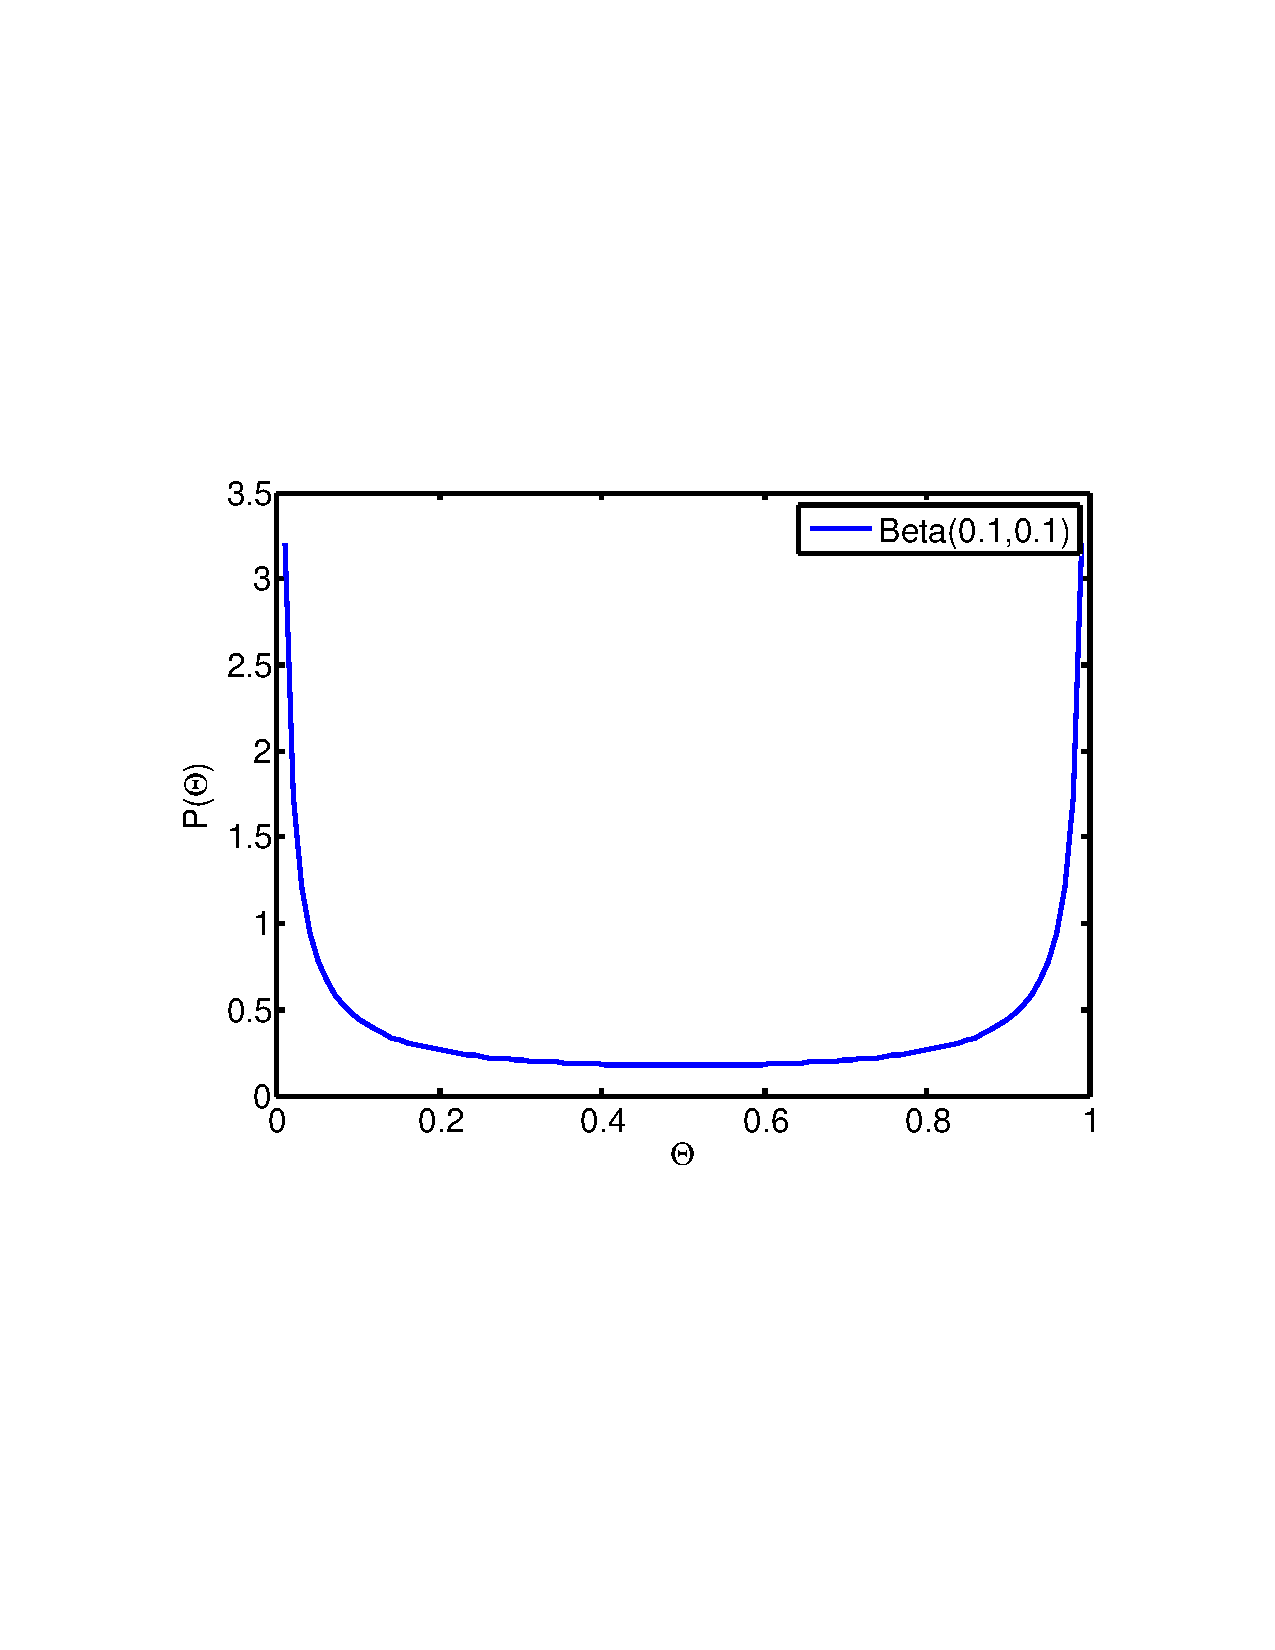
\includegraphics[width=.5\textwidth]{../introduction_to_bayes/beta_p1_p1.pdf} % requires the graphicx package
\caption{Beta(.1,.1)}
\end{center}
\end{figure}


}


\frame[t] {% slide 8
\frametitle{Beta Distribution}
\begin{figure}[htbp]
\begin{center}
 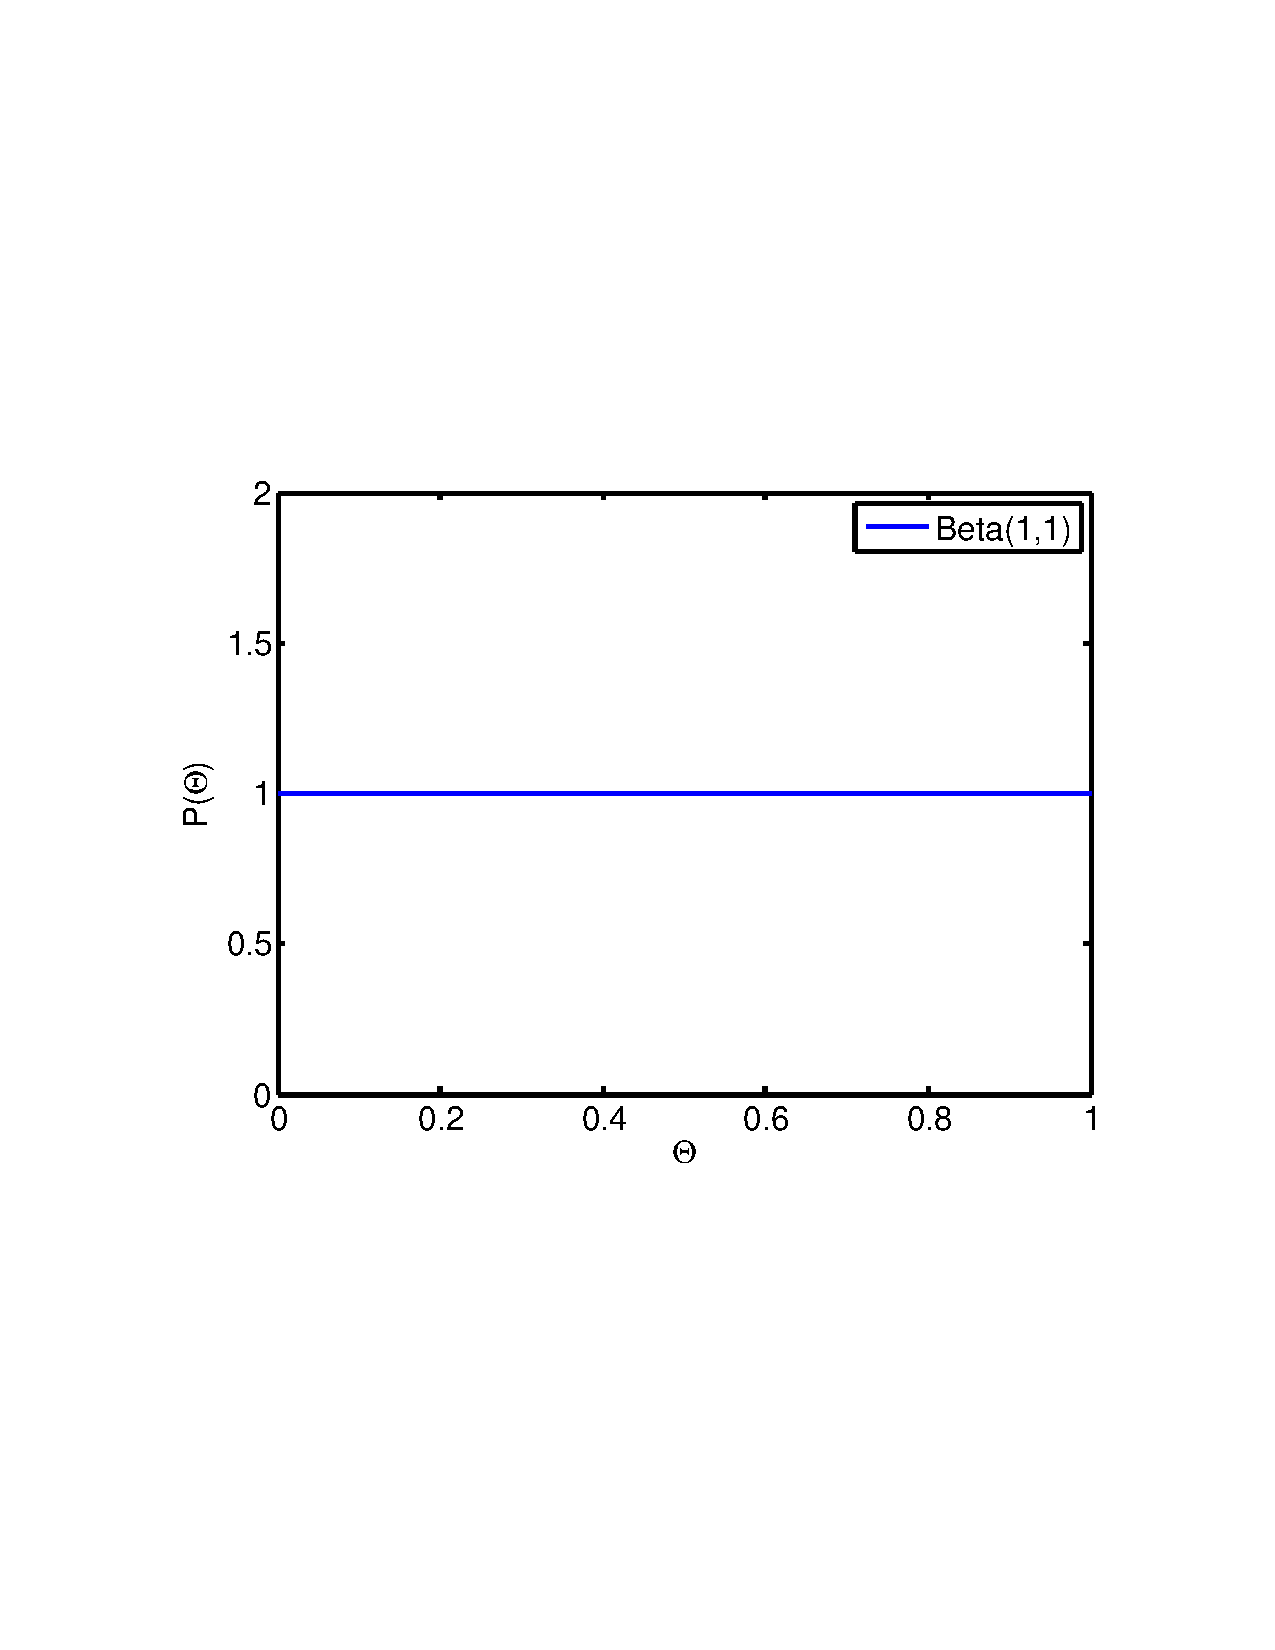
\includegraphics[width=.5\textwidth]{../introduction_to_bayes/beta_1_1.pdf} % requires the graphicx package
\caption{Beta(1,1)}
\end{center}
\end{figure}


}

\frame[t] {% slide 8
\frametitle{Beta Distribution}
\begin{figure}[htbp]
\begin{center}
 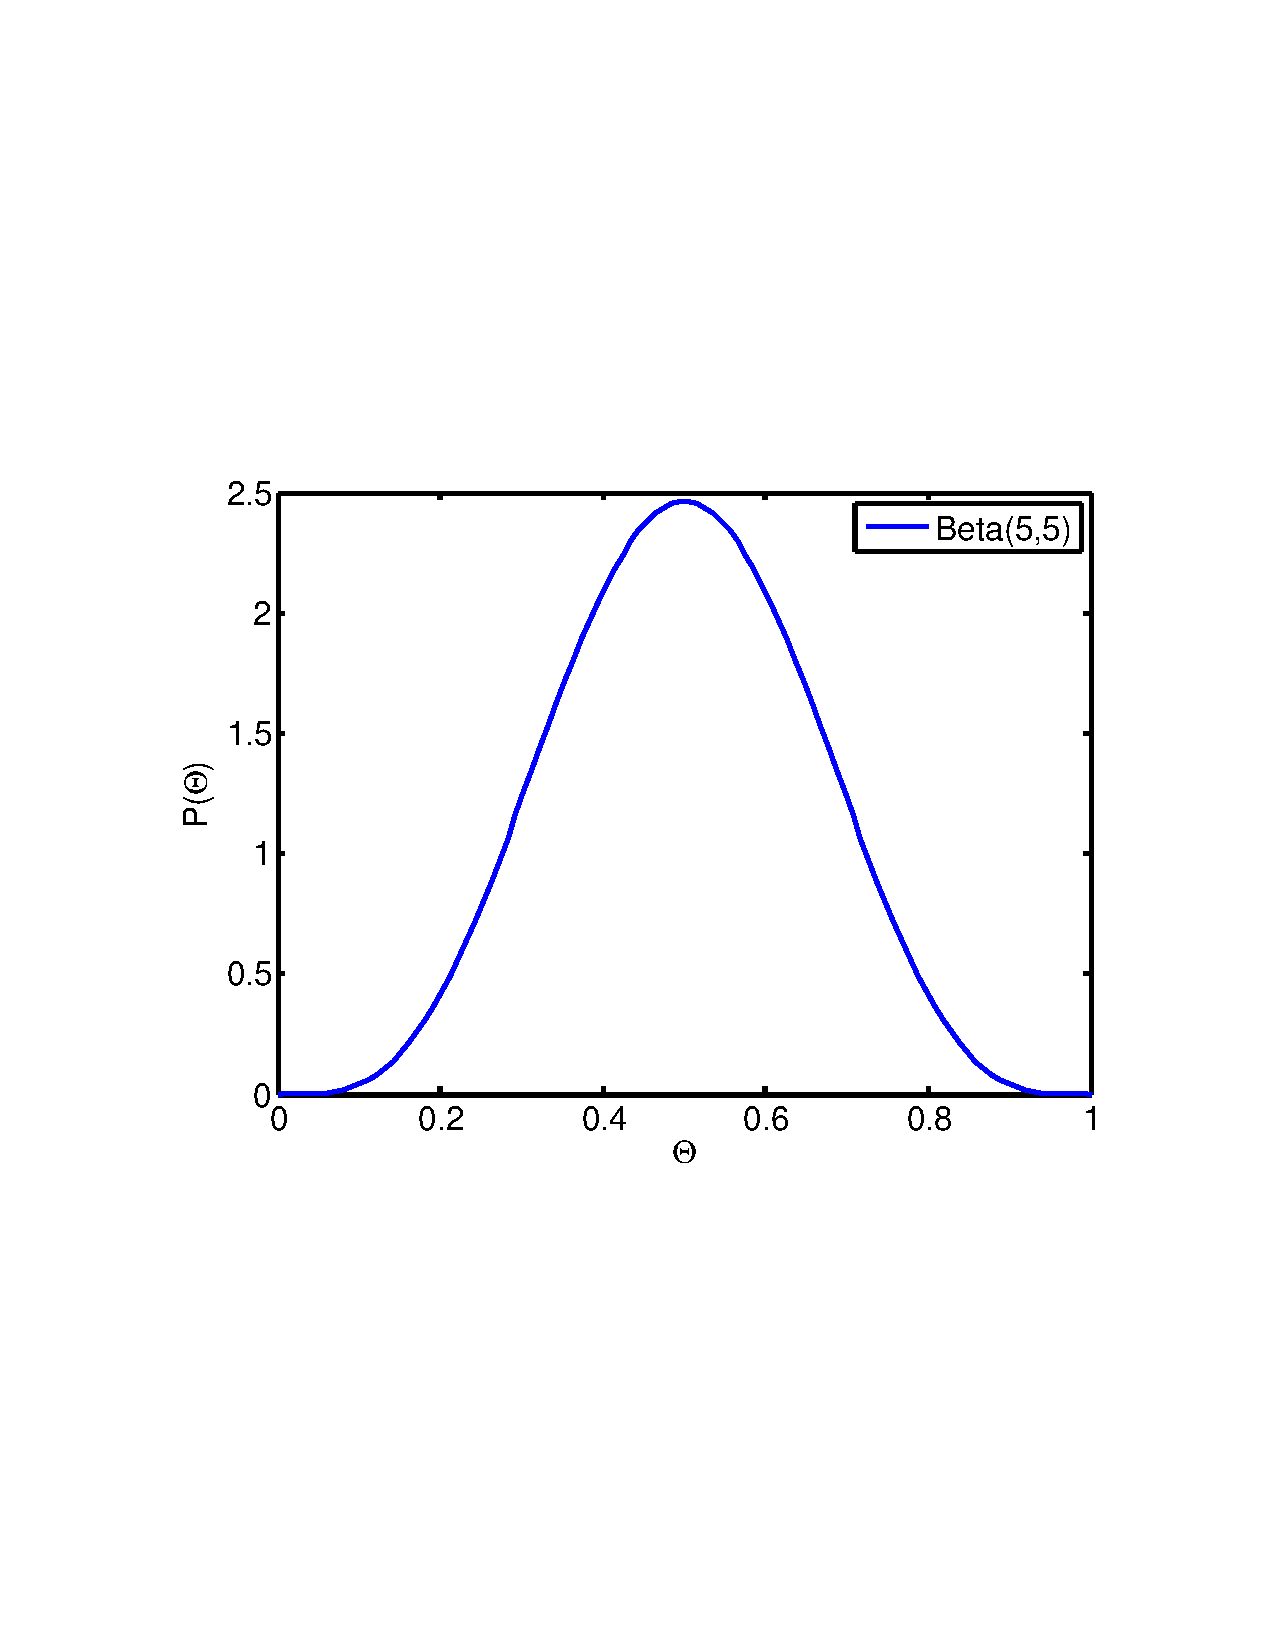
\includegraphics[width=.5\textwidth]{../introduction_to_bayes/beta_5_5.pdf} % requires the graphicx package
\caption{Beta(5,5)}
\end{center}
\end{figure}


}

\frame[t] {% slide 8
\frametitle{Beta Distribution}
\begin{figure}[htbp]
\begin{center}
 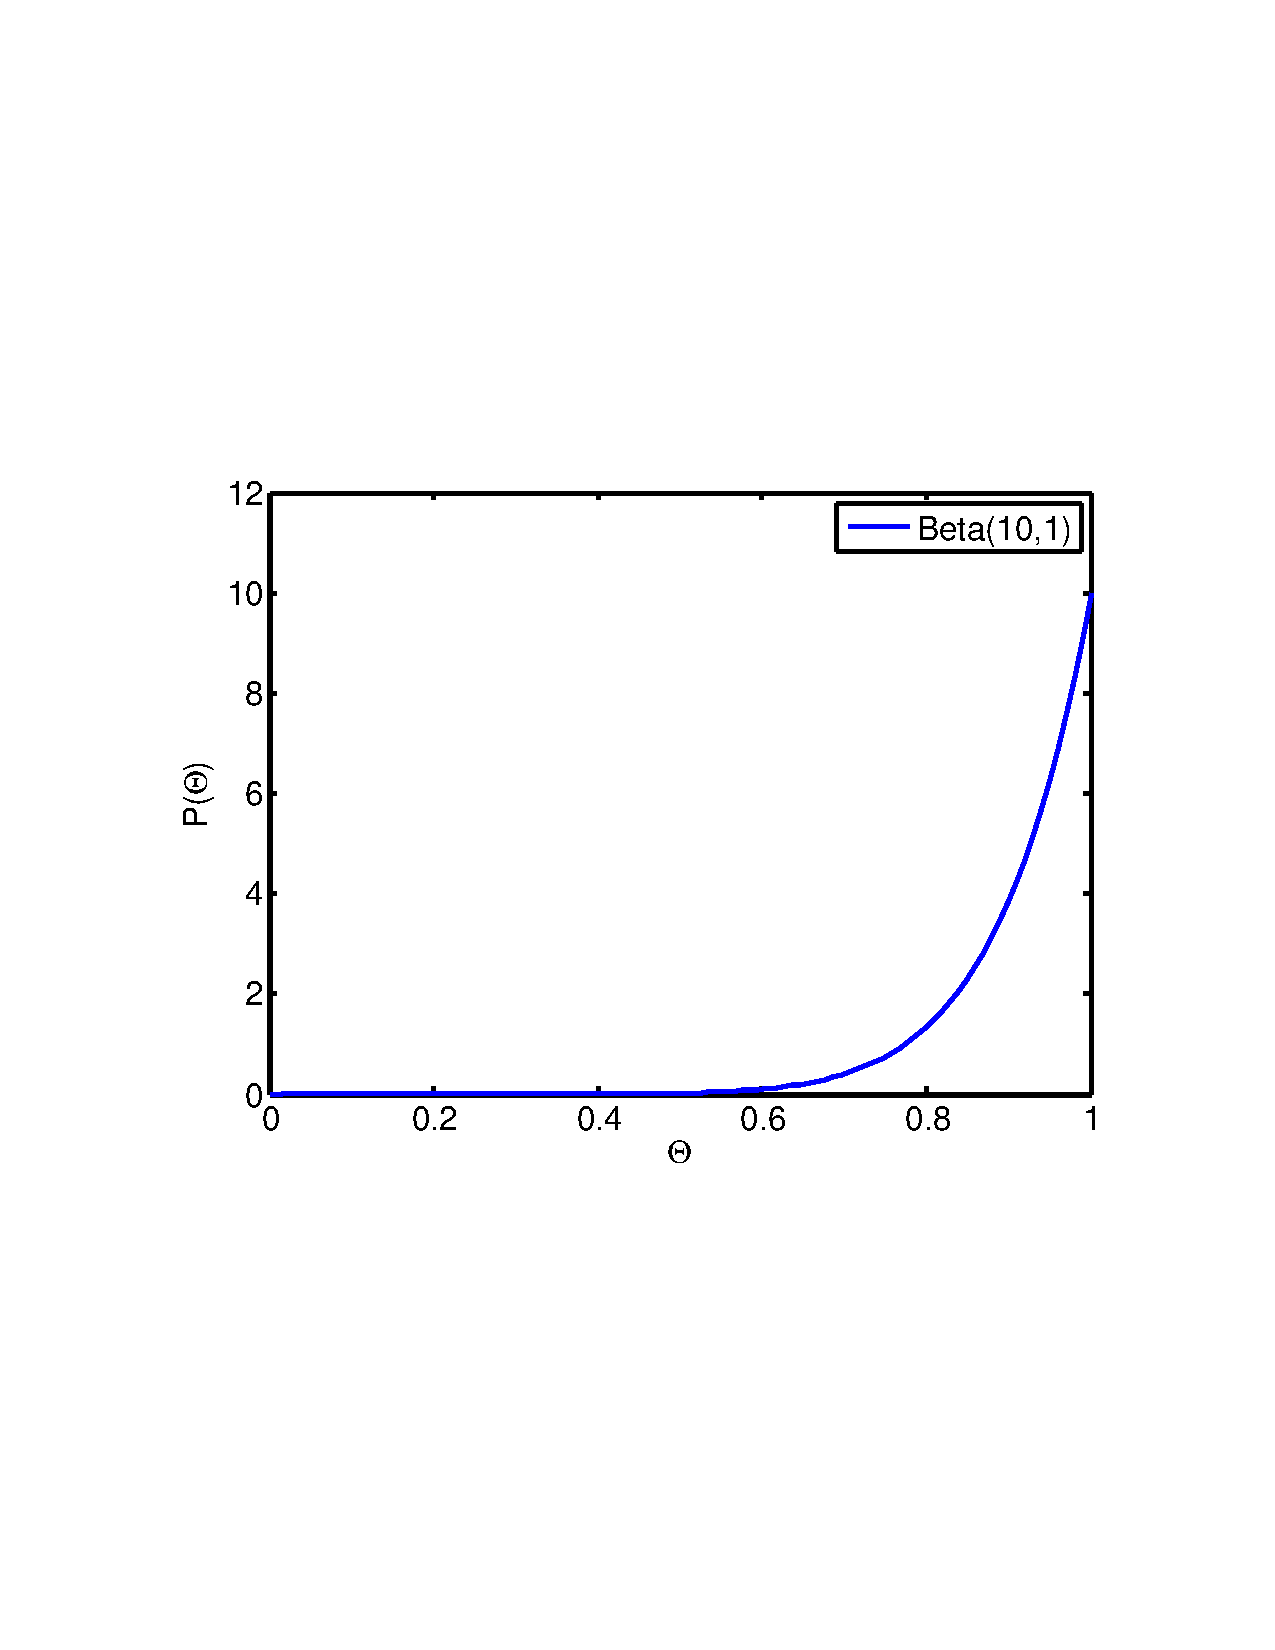
\includegraphics[width=.5\textwidth]{../introduction_to_bayes/beta_10_1.pdf} % requires the graphicx package
\caption{Beta(10,1)}
\end{center}
\end{figure}


}

\frame[t] {% slide 8
\frametitle{Generative Model}
With the introduction of this prior we now have a full generative model of our data (given $\alpha$ and $\beta$, the model's hyperparameters).  

Consider the following procedure for generating pencil failure data:

\begin{itemize}
\item Sample a failure rate parameter $\Theta$ for the ``factory'' from a $\Bet(\alpha, \beta)$ distribution.  This yields the failure rate for the factory.
\item Given the failure rate $\Theta$, sample $N$ defect/no-defect observations from a Bernoulli distribution with parameter $\Theta.$
\end{itemize}

Bayesian inference involves ``turning around'' this generative model, i.e.~uncovering a distribution over the parameter $\Theta$ given both the observations and the prior.

}


\frame[t] {% slide 8
\frametitle{Inferring the Posterior Distribution}

Remember that the {\em posterior distribution} of the model parameters is given by \[P(\Theta| X_1,\ldots, X_n) \propto P( X_1,\ldots,
X_n|\Theta) P(\Theta) \] 
Let's consider what the posterior looks like after observing a single observation (in our example). \newline

Our likelihood is given by \[ P( X_1|\Theta) = \Theta^{X_1}(1-\Theta)^{1-X_1}\]

Our prior, the Beta distribution, is given by 
\[ P(\Theta) = \frac{\Gamma(\alpha+\beta)}{\Gamma(\alpha)\Gamma(\beta)}\Theta^{\alpha-1}(1-\Theta)^{\beta-1}\]
}

\frame[t] {% slide 8
\frametitle{Posterior Update Computation}

Since we know that \[P(\Theta| X_1) \propto P( X_1|\Theta) P(\Theta) \] we can write 

 \[P(\Theta| X_1) \propto  \Theta^{X_1}(1-\Theta)^{1-X_1} \frac{\Gamma(\alpha+\beta)}{\Gamma(\alpha)\Gamma(\beta)}\Theta^{\alpha-1}(1-\Theta)^{\beta-1}\]
 but since we are interested in a function (distribution) of $\Theta$ and we are working with a proportionality, we can throw away terms that do not involve $\Theta$ yielding
 \[P(\Theta| X_1) \propto   \Theta^{\alpha+X_1-1}(1-\Theta)^{1-X_1+\beta-1}\]
}

\frame[t] {% slide 8
\frametitle{Bayesian Computation, Implicit Integration}
From the previous slide we have
 \[P(\Theta| X_1) \propto   \Theta^{\alpha+X_1-1}(1-\Theta)^{1-X_1+\beta-1}\]
To make this proportionality an equality (i.e.~to construct a properly normalized distribution) we have to integrate this expression w.r.t.~$\Theta$, i.e.
 \[P(\Theta| X_1) =  \frac{\Theta^{\alpha+X_1-1}(1-\Theta)^{1-X_1+\beta-1}}{\int \Theta^{\alpha+X_1-1}(1-\Theta)^{1-X_1+\beta-1} d\Theta}\]
 But in this and other special cases like it (when the likelihood and the prior form a conjugate pair) this integral can be solved by recognizing the form of the distribution, i.e.~note that this expression looks exactly like a Beta distribution but with updated parameters, $\alpha_1 = \alpha+X_1, \beta_1 = \beta + 1 - X_1$
 }
 
\frame[t] {% slide 8
\frametitle{Posterior and Repeated Observations}

This yields the following pleasant result

\[\Theta | X_1, \alpha, \beta \sim \Bet(\alpha+X_1, \beta + 1 - X_1)\]

This means that the posterior distribution of $\Theta$ given an observation is in the same parametric family as the prior.  This is characteristic of conjugate  likelihood/prior pairs.  \newline

Note the following decomposition

\[ P(\Theta | X_1, X_2, \alpha, \beta) \propto P(X_2| \Theta, X_1) P(\Theta | X_1, \alpha, \beta)  \]

This means that the preceding posterior update procedure can be repeated.  This is because $P(\Theta | X_1, \alpha, \beta)$ is in the same family (Beta) as the original prior.  The posterior distribution of $\Theta$ given two observations will still be Beta distributed, now just with further updated parameters.
 }
 
 \frame[t] {% slide 8
\frametitle{Incremental Posterior Inference}

Starting with 

\[\Theta | X_1, \alpha, \beta \sim \Bet(\alpha+X_1, \beta + 1 - X_1)\]

and adding $X_2$ we can almost immediately identify 

\[\Theta | X_1, X_2, \alpha, \beta \sim \Bet(\alpha+X_1+X_2, \beta + 1 - X_1 +1 -X_2)\]

which simplifies to 

\[\Theta | X_1, X_2, \alpha, \beta \sim \Bet(\alpha+X_1+X_2, \beta + 2 - X_1 -X_2)\]

and generalizes to 

\[\Theta | X_1, \ldots, X_N, \alpha, \beta \sim \Bet(\alpha+\sum X_i, \beta + N -\sum X_i)\]
 }
 
\frame[t] {% slide 8
\frametitle{Interpretation, Notes, and Caveats}
\begin{itemize}
\item The posterior update computation performed here is unusually simple in that it is analytically tractable.  The integration necessary to normalize the posterior distribution is more often not analytically tractable than it is analytically tractable.  When it is not analytically tractable other methods must be utilized to get an estimate of the posterior distribution -- numerical integration and Markov chain Monte Carlo (MCMC) amongst them.
\item The posterior distribution can be interpreted as the distribution of the model parameters given both the structural assumptions made in the model selection step and the selected prior parameterization.  Asking questions like, ``What is the probability that the factory has a defect rate of less than 10\%?'' can be answered through operations on the posterior distribution.
\end{itemize}

 }
 
 \frame[t] {% slide 8
\frametitle{More Interpretation, Notes, and Caveats}
The posterior can be seen in multiple ways
\begin{eqnarray*}
 P(\Theta| X_{1:N}) &\propto& P( X_1,\ldots,
X_N|\Theta) P(\Theta) \\
&\propto& P( X_N | X_{1:N-1},\Theta) P(X_{N-1} | X_{1:N-2},\Theta) \cdots P(X_{1}|\Theta) P(\Theta) \\
&\propto& P( X_N | \Theta) P(X_{N-1}|\Theta) \cdots P(X_{1}|\Theta) P(\Theta) 
\end{eqnarray*}
(when $X$'s are iid given $\Theta$ or exchangeable) and
\begin{eqnarray*}
 P(\Theta| X_1,\ldots, X_N) &\propto& P( X_N,\Theta | X_1\ldots, X_{N-1})\\
&\propto&  P( X_N|\Theta) P(\Theta | X_1\ldots, X_{N-1})\\
\end{eqnarray*}

The first decomposition highlights the fact that the posterior distribution is influenced by each observation. \newline

The second recursive decomposition highlights the fact that the posterior distribution can be interpreted as the full characterization of the uncertainty about the hidden parameters after having  accounted for all observations to some point.
 }
 
  \frame[t] {% slide 8
\frametitle{Posterior Predictive Inference}
Now that we know how to update our prior beliefs about the state of latent variables in our model we can consider posterior predictive inference.  \newline

Posterior predictive inference performs a weighted average prediction of future values over all possible settings of the model parameters.  The prediction is weighted by the posterior probability of the model parameter setting, i.e.

\[P(X_{N+1} | X_{1:N} ) = \int P(X_{N+1} | \Theta) P(\Theta | X_{1:N})d\Theta\]

Note that this is just the likelihood convolved against the posterior distribution having accounted for $N$ observations.
 }
 
   \frame[t] {% slide 8
\frametitle{More Implicit Integration}
If we return to our example we have the updated posterior distribution
\[\Theta | X_1, \ldots, X_N, \alpha, \beta \sim \Bet(\alpha+\sum_{i=1}^N X_i, \beta + N -\sum_{i=1}^N X_i)\]
and the likelihood of the $(N+1)^{th}$ observation
\[ P( X_{N+1}|\Theta) = \Theta^{X_{N+1}}(1-\Theta)^{1-X_{N+1}}\]
Note that the following integral is similar in many ways to the posterior update
\[P(X_{N+1} | X_{1:N} ) = \int P(X_{N+1} | \Theta) P(\Theta | X_{1:N})d\Theta\]
which means that in this case (and in all conjugate pairs) this is easy to do.
 }
 
    \frame[t] {% slide 8
\frametitle{More Implicit Integration}

\begin{eqnarray*}
P(X_{N+1} | X_{1:N} )& =& \int\Theta^{X_{N+1}}(1-\Theta)^{1-X_{N+1}} \\
&\times& \frac{\Gamma(\alpha+\beta + N)}{\Gamma(\alpha+\sum_{i=1}^N X_i)\Gamma(\beta + N -\sum_{i=1}^N X_i)} \\
&\times& \Theta^{\alpha+\sum_{i=1}^N X_i-1}(1-\Theta)^{\beta + N -\sum_{i=1}^N X_i)-1}d\Theta
\end{eqnarray*}
\begin{eqnarray*}
& =&  \frac{\Gamma(\alpha+\beta + N)}{\Gamma(\alpha+\sum_{i=1}^N X_i)\Gamma(\beta + N -\sum_{i=1}^N X_i)} \\
&\times&  \frac{\Gamma(\alpha+\sum_{i=1}^N X_i + X_{N+1})\Gamma(\beta + N+1 -\sum_{i=1}^N X_i - X_{N+1})}{\Gamma(\alpha+\beta + N+1)} \\
\end{eqnarray*}
 }
 
     \frame[t] {% slide 8
\frametitle{Interpretation}
\begin{eqnarray*}
\lefteqn{P(X_{N+1} | X_{1:N} )}\\
 &=&  \frac{\Gamma(\alpha+\beta + N)}{\Gamma(\alpha+\sum_{i=1}^N X_i)\Gamma(\beta + N -\sum_{i=1}^N X_i)} \\
&\times&  \frac{\Gamma(\alpha+\sum_{i=1}^N X_i + X_{N+1})\Gamma(\beta + N+1 -\sum_{i=1}^N X_i - X_{N+1})}{\Gamma(\alpha+\beta + N+1)} \\
\end{eqnarray*}
 Is a ratio of Beta normalizing constants. \newline
 
 This a distribution over $[0,1]$ which averages over all possible models in the family under consideration (again, weighted by their posterior probability). 

 }
 
      \frame[t] {% slide 8
\frametitle{Caveats again}
In posterior predictive inference many of the same caveats apply.  

\begin{itemize}
\item Inference can be computationally demanding if conjugacy isn't exploited.
\item Inference results are only as good as the model and the chosen prior.  
\end{itemize}
But Bayesian inference has some pretty big advantages
\begin{itemize}
\item Assumptions are explicit and easy to characterize.
\item It is easy to plug and play Bayesian models.
\end{itemize}

 }
 
 
\frame[t] {% slide 8
\frametitle{Beta Distribution}
\begin{figure}[htbp]
\begin{center}
 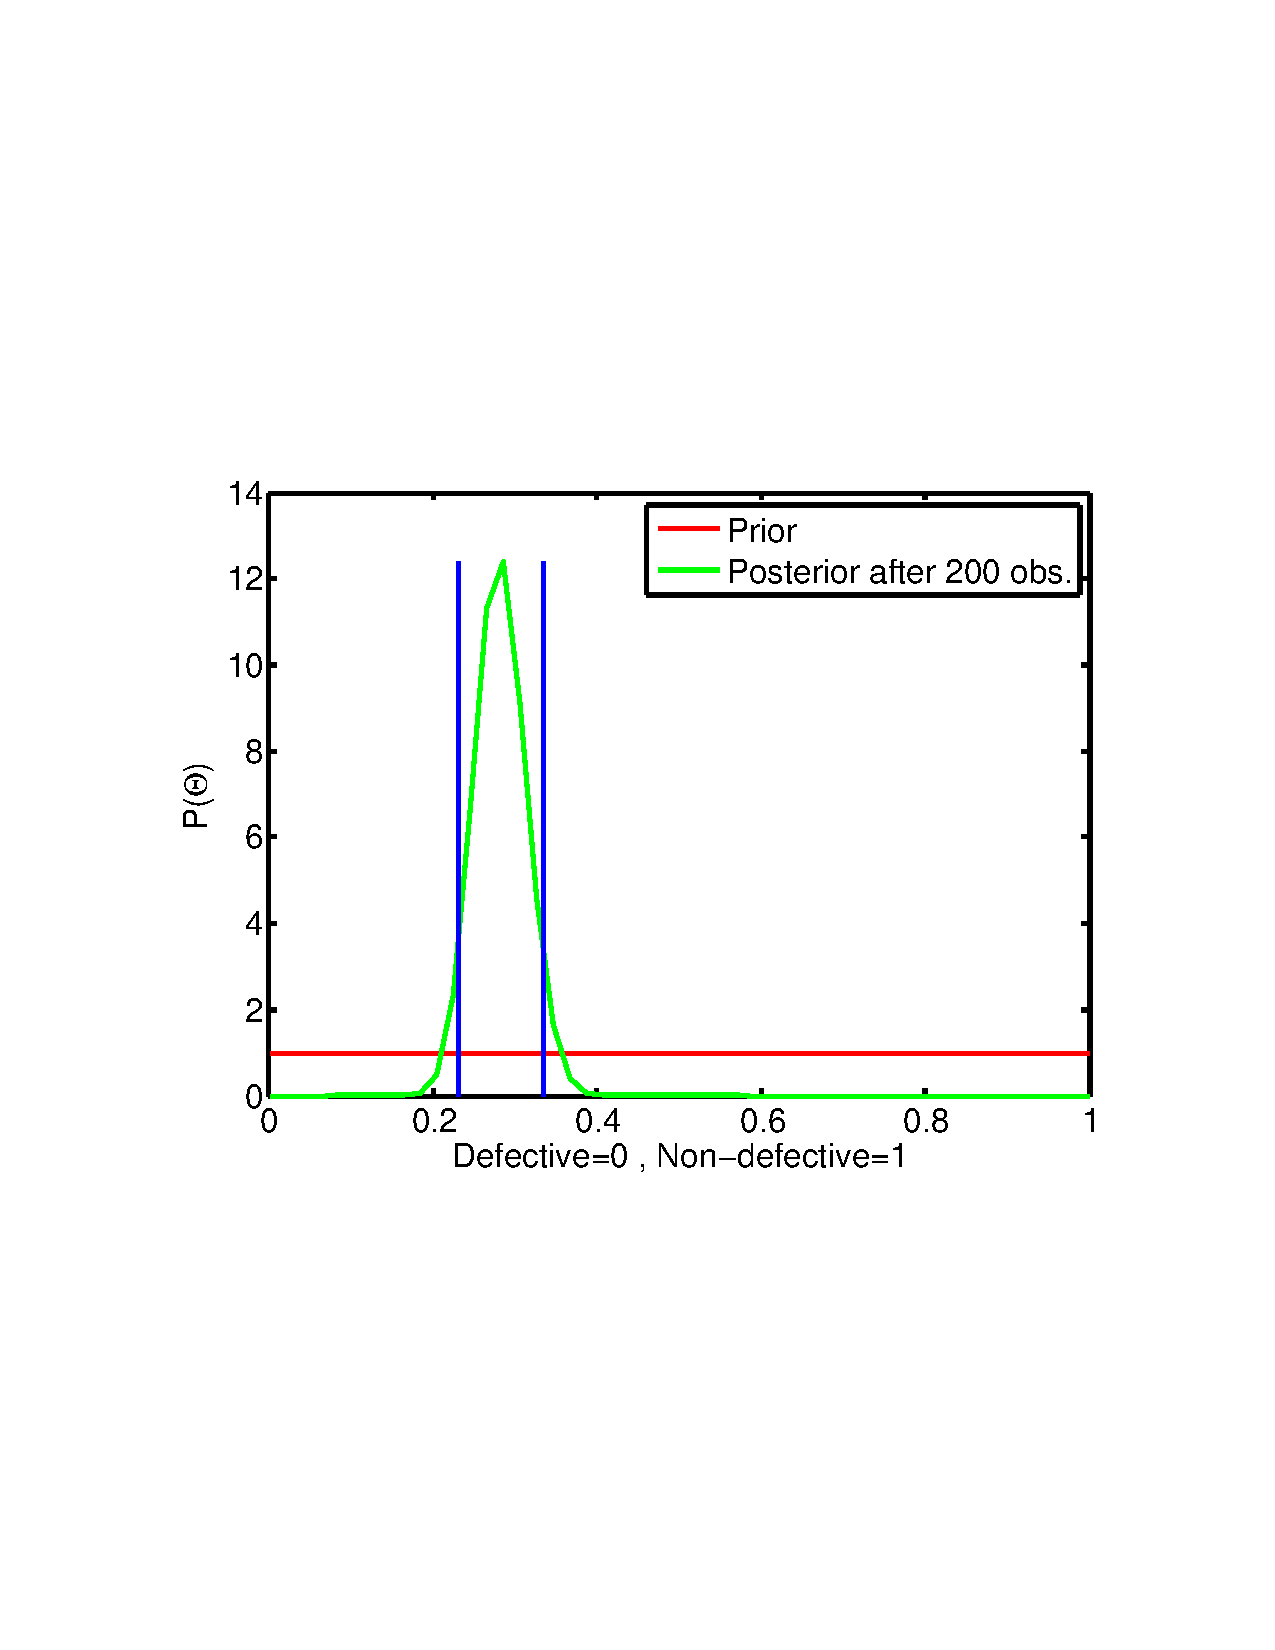
\includegraphics[width=.5\textwidth]{../introduction_to_bayes/posterior.pdf} % requires the graphicx package
\caption{Posterior after 1000 observations.}
\end{center}
\end{figure}


}


\frame[t] {% slide 8
\frametitle{Beta Distribution}
\begin{figure}[htbp]
\begin{center}
 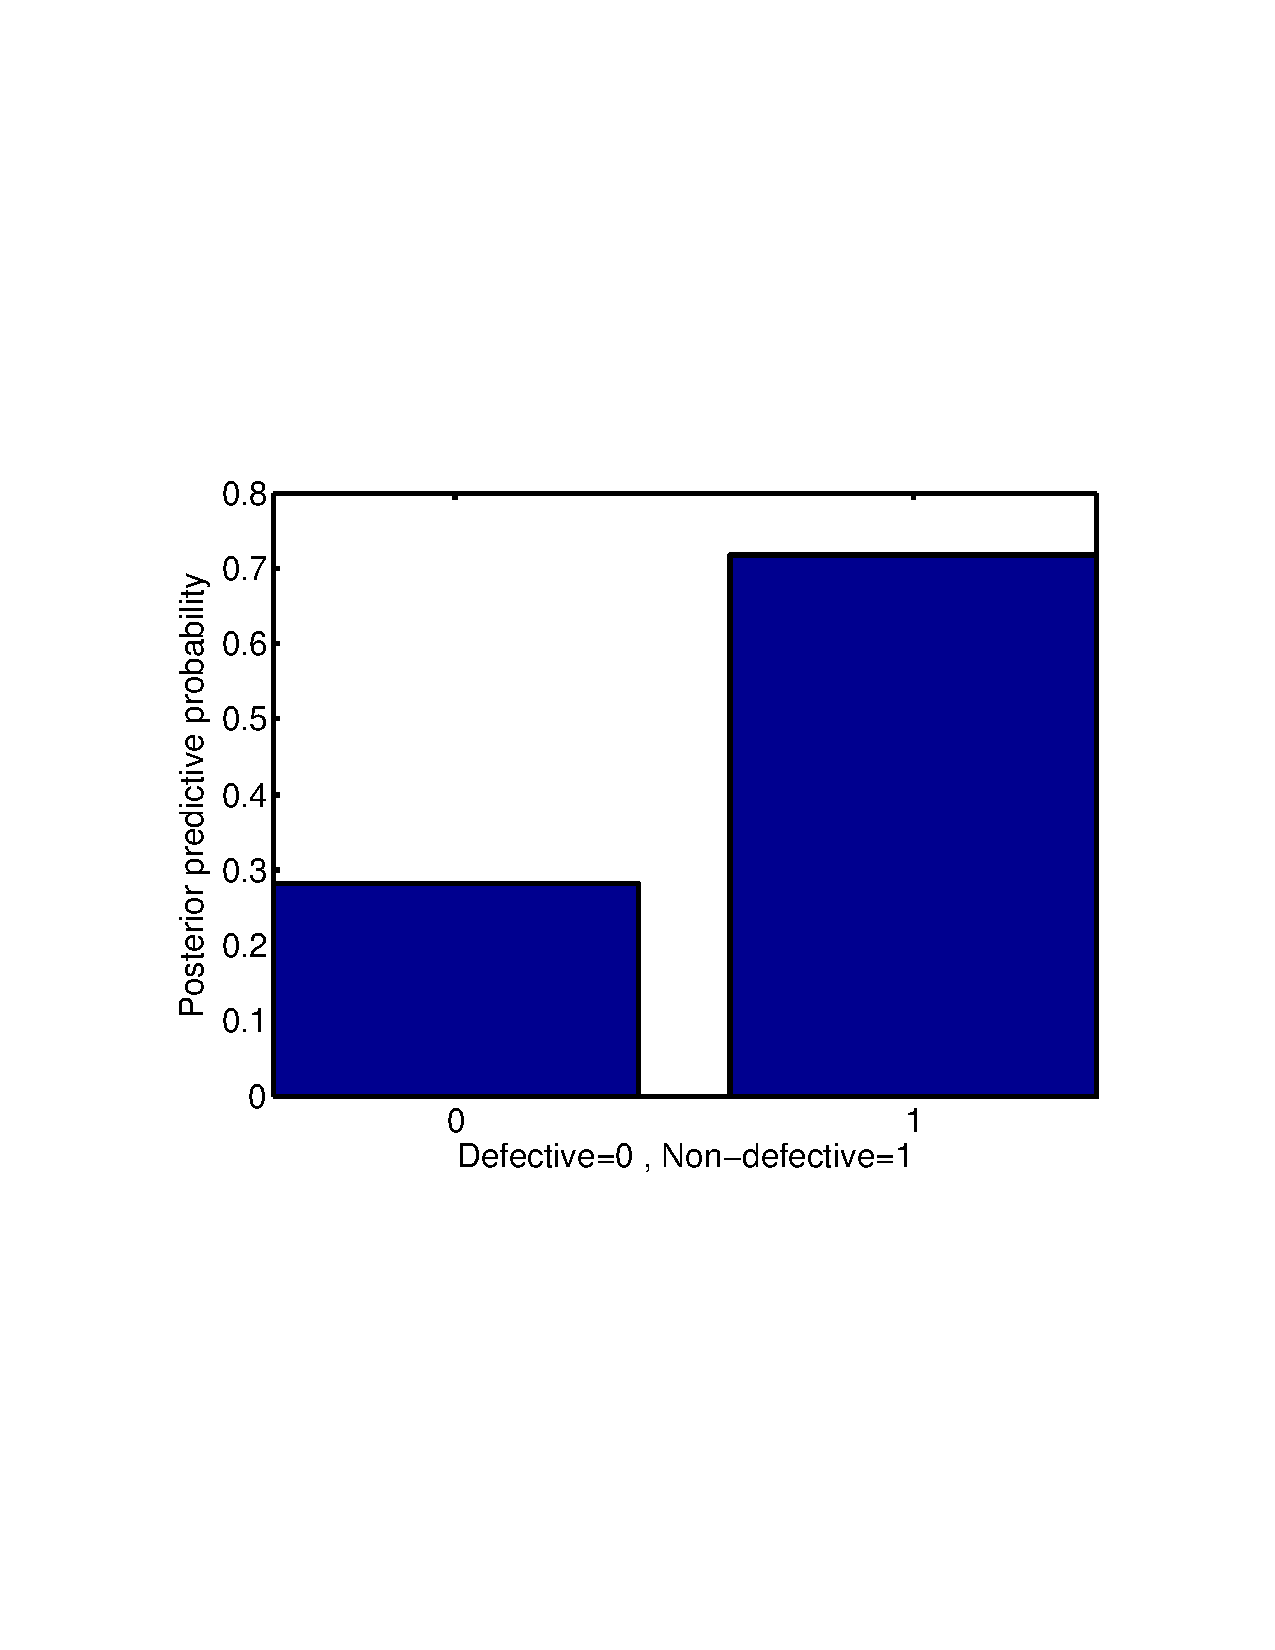
\includegraphics[width=.5\textwidth]{../introduction_to_bayes/posterior_predictive.pdf} % requires the graphicx package
\caption{Posterior predictive after 1000 observations.}
\end{center}
\end{figure}


}

 


\end{document}
